\section{Evaluation}
The evaluation of the clustering algorithms was performed on a Intel i7 1.70 GHz processor (12th gen.) with 16 GB of RAM running Windows 11.

The evaluation of MAFIA was performed using \textit{GPUMAFIA} \cite{gpumafia}, which was installed on a virtual machine(VM) running Ubuntu 24.04.1 LTS using VirtualBox. The VM was configured with 4 CPUs and 4 GB of RAM. In contrast, CLIQUE and SUBCLU were evaluated on the main machine (host) using ELKI \cite{elki}. Thus, one should be careful to compare the results of MAFIA with those of CLIQUE and SUBCLU, as the execution environment may affect the results, however, their growth rate can be compared.

The evaluation project can be found at the GitHub repository: \url{https://github.com/henrikdchristensen/SDU-Data-Mining-Exam}, where additional tests can be found as well as detailed descriptions of how to generate the data sets and how to install and use GPUMAFIA.

\subsection{Data set generation}
The aim for synthetic data generation was to be able to produce similar data sets as discussed in \cite{mafia}. Using \textit{MDCGen} it was possible to create large high-dimensional axis-parallel clustered data sets. Here, for example, the number of dimensions, number of clusters, number of data points and percentage of noise can be specified. Furthermore, it was possible to determine for each cluster which of the dimensions that are noise. Also, all dimensions ranges from 0 to 1, as assumed for both MAFIA and SUBCLU.

However, to see the difference between CLIQUE and MAFIA against the SUBCLU algorithm, a data set containing a Bezier-shaped cluster was created using \textit{Artificial Cluster} (AC). Also, a home-made data set containing a plus-shaped cluster was created as discussed in \cite{mafia}

\subsection{Experimental Results}

\subsubsection{Scalability with Data Set Size}
Figure \ref{fig:dataset_size_vs_runtime} shows the scalability of the three algorithms with increasing data set size. The data set contains 20 dimensions with 5 clusters in 5 different subspaces with 10\% noise records. The data set size ranges from 10k to 15mio records. However, only MAFIA was able to handle the full amount of data. CLIQUE was able to handle up to 7mio records, while SUBCLU was only able to handle up to 200k records. The results clearly shows that MAFIA is the most scalable algorithm, followed by CLIQUE and SUBCLU.

\begin{figure}
    \centering
    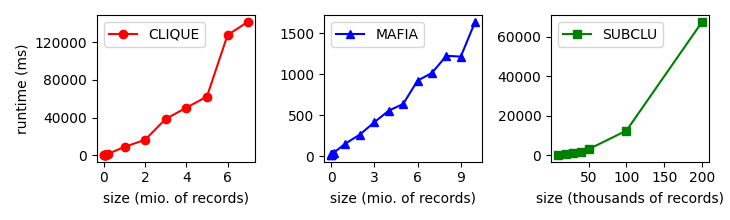
\includegraphics[scale=0.6]{figures/dataset_size_vs_runtime.png}
    \caption{Scalability with increasing data set size.}
    \label{fig:dataset_size_vs_runtime}
\end{figure}

\subsubsection{Clustering Accuracy}
Different data sets were generated to test the clustering accuracy of the algorithms.

The first data set were a 2-dimensional data set containing a single cluster formed as a plus, see Figure \ref{fig:accuracy_plus}. Same results were reproduced as found in \cite{mafia}, however, it must be noted that for MAFIA to be able to detect the 2-dimensional cluster, it will report some lower-dimensional clusters as well. In contrast, CLIQUE was only able to partly detect the cluster.
\begin{figure}
    \centering
    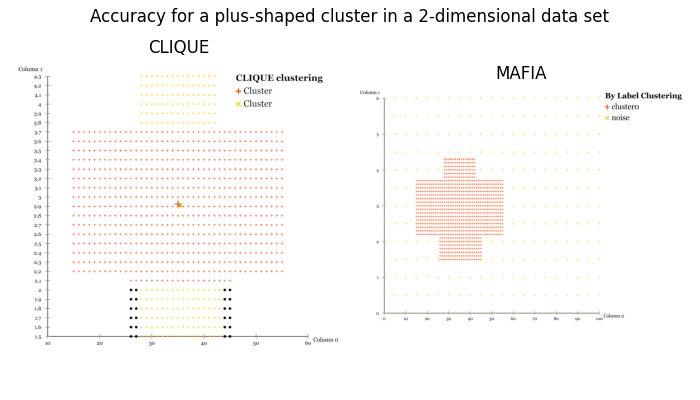
\includegraphics[scale=0.45]{figures/accuracy_plus.png}
    \caption{Plus-shaped cluster.}
    \label{fig:accuracy_plus}
\end{figure}

The second data set were a 2-dimensional data set containing a single cluster formed as a Bezier curve, see Figure \ref{fig:accuracy_bezier}. The results were similar to the plus-shaped cluster, however, CLIQUE was able to detect the cluster, but not as accurate as MAFIA.

\begin{figure}
    \centering
    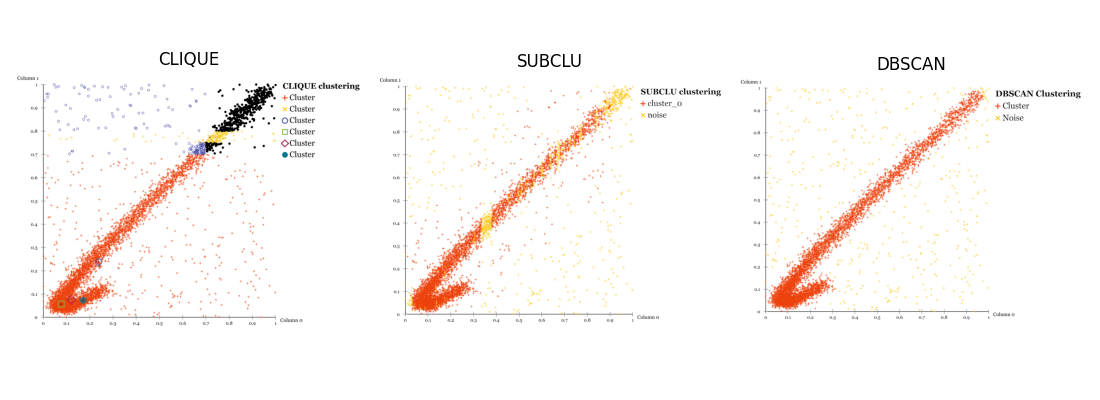
\includegraphics[scale=0.45]{figures/accuracy_bezier.png}
    \caption{Bezier-shaped cluster.}
    \label{fig:accuracy_bezier}
\end{figure}

The third data set were a 10-dimensional data set. 10\% of the data was added as noise records.

\begin{figure}
    \centering
    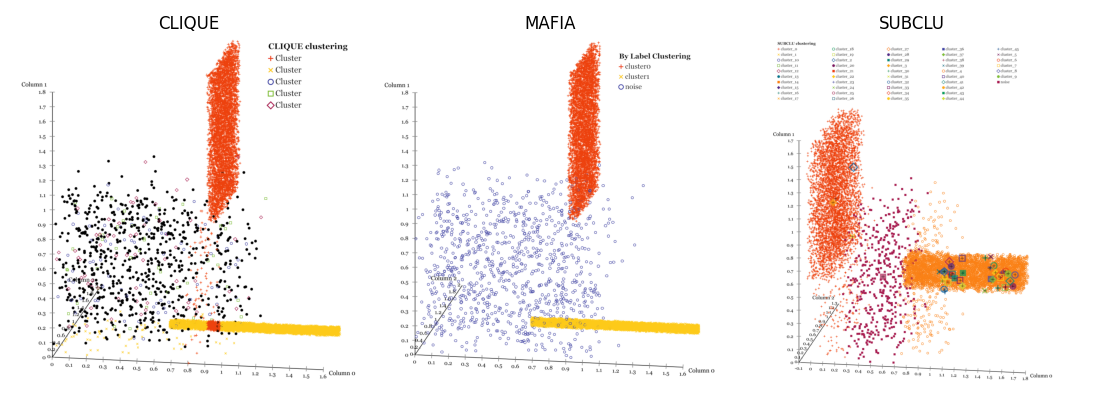
\includegraphics[scale=0.45]{figures/accuracy_2clusters.png}
    \caption{Clusters in different subspaces.}
    \label{fig:accuracy_2clusters}
\end{figure}

\subsubsection{Scalability with Data Dimensionality and Cluster Dimensionality}
Figure \ref{fig:dataset_dimensionality_vs_runtime} shows the scalability of the CLIQUE and MAFIA with increasing data set dimensionality. The data set contains 1 mio. records with 5 clusters in 5 different subspaces and 10\% noise records. The data set dimensionality ranges from 10 to 100 dimensions. The results clearly shows that MAFIA is the most scalable algorithm.

Figure \ref{fig:cluster_dimensionality_vs_runtime} shows the scalability of the CLIQUE and MAFIA with increasing cluster dimensionality. The data set contains 500k records with 5 clusters in 5 different subspaces with 10\% noise records. The data set dimensionality is 20 dimensions. The cluster dimensionality ranges from 10 to 100 dimensions. The results clearly shows that MAFIA is the most scalable algorithm.
\begin{figure}
    \centering
    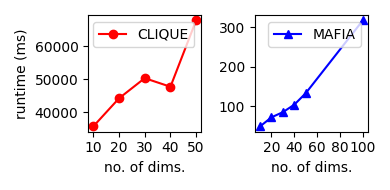
\includegraphics[scale=0.6]{figures/data_dimensionality_vs_runtime.png}
    \caption{Scalability with increasing data set dimensionality.}
    \label{fig:dataset_dimensionality_vs_runtime}
\end{figure}

\begin{figure}
    \centering
    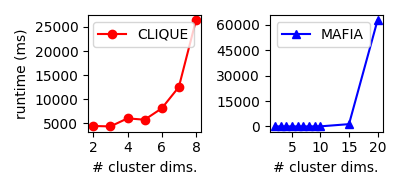
\includegraphics[scale=0.6]{figures/cluster_dimensionality_vs_runtime.png}
    \caption{Scalability with increasing cluster dimensionality.}
    \label{fig:cluster_dimensionality_vs_runtime}
\end{figure}

The results reported for SUBCLU \cite{subclu} were also tried to be replicated, however, similar results were not achieved.

\subsection{Sensitive analysis for MAFIA}
\begin{figure}
    \centering
    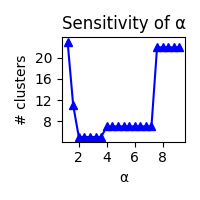
\includegraphics[scale=0.6]{figures/sensitivity_alpha.png}
    \caption{Sensitive analysis for MAFIA.}
    \label{fig:sensitivity_alpha}
\end{figure}

\subsubsection{Real Data Sets}